%\documentclass{article}
\documentclass[10pt]{article}
\usepackage{times}
%\usepackage{natbib}
%\usepackage{multicol}
\RequirePackage{natbib}
\usepackage{amsmath, amssymb, fullpage, amsthm, array,,graphicx,asa, url}
%\usepackage[dvips]{graphics}

%\usepackage{hyperref} % for hyper reference

\graphicspath{{images/}}

% \usepackage{pifont} % this package is used to print check mark \checkmark
% \linespread{1.6} % factor 1.6 = double space

%\usepackage{setspace}
%\doublespacing



\setlength{\oddsidemargin}{0in}
\setlength{\evensidemargin}{0in}
\setlength{\textwidth}{6.5in}
\setlength{\topmargin}{-0.4in}
\setlength{\textheight}{9in}
\evensidemargin 
\oddsidemargin

\newtheorem{thm}{Theorem}[section]
\newtheorem{dfn}{Definition}[section]
\newtheorem{cor}{Corollary}[thm]
\newtheorem{con}{Conjecture}[thm]
\newtheorem{lemma}[thm]{Lemma}

%\topmargin -0.10in   % when making pdf
%\textheight 9.15in  % when making pdf

\pdfminorversion=4 % as instructed by JASA file upload


\begin{document}

\tableofcontents

% Article top matter
\title{Impact of Demographics and Skills of the Observer on Visual Statistical Inference }
\author{{Mahbubul Majumder, Heike Hofmann, Dianne Cook}
\thanks{Mahbubul Majumder is a PhD student (e-mail: mahbub72@gmail.com) , Heike Hofmann is an Associate  Professor and Dianne Cook is a Professor in the Department of Statistics and Statistical Laboratory, Iowa State University, Ames, IA 50011-1210. This research is supported in part by the National Science Foundation Grant \# DMS 1007697.}}
\date{\vspace{-.5in}}
%\date{\today}  %\today is replaced with the current date
\maketitle

\begin {abstract}  
Visual Statistical Inference is dependent on the careful evaluation of the lineups by individual observers. Each individual is different in their cognitive phycology and judiciousness which can affect the power of visual inference. To estimate the power of visual inference this can be controlled by getting evaluations from multiple people from a diverse population. But the other factor that may affect the power of visual inference is the demographics and skills of the observer. In this paper we examine this in details. The simulation experiments suggest that individual skill as well as demographics are very significant for the power of visual inference. We examine the evidence of learning or getting skilled while sequentially evaluating multiple lineups which enables them evaluate a lineup faster in the later attempts. The experimental data suggest that there is no learning effect in terms of correct response. The location of actual plot in the lineups does not have any significant effect as well.

{\bf Keywords: \sf statistical graphics, lineup, non-parametric test, cognitive phycology, visualization, exploratory data analysis} 
\end {abstract}

%\begin{multicols}{2}
%\twocolumn

\section{Introduction}  

Statistical graphics can be used to test the significance of findings during the exploratory data analysis. The method is now termed as visual statistical inference which is discussed in the following section.

\subsection{Visual Statistical Inference} The fundamental concept of visual statistical inference is introduced by \citet{buja:2009}. In their paper, they proposed lineup protocol to discover significant pattern in the data. Later these concepts are further developed by defining necessary terminologies and validating using a head to head comparison with conventional inference by \citet{majumder:2013}. The power of the visual test is obtained and it is observed that the power is as good as conventional test while in some scenarios, the power exceeds the conventional test power.

The test statistic used in visual inference is a plot of the data. This plot is then placed on a layout of plot called lineup. The rest of the plots in a lineup are generated from the model specified by the null hypothesis. An observer is then asked to evaluate the lineup. If the observer can detect the observed plot in the lineup, the hypothesis is rejected. Figure \ref{fig:lineup_geno} displays a lineup of 20 plots where one of the plots is observed data. The rest of the 19 plots are generated from the assumption that there is no difference between two groups of data. For this, the group structure of the data is broken by random permutation of the groups. If the null hypothesis is true, the observed data should look similar to the rest of the plots in the lineup making it difficult to detect the observed plot. On the other hand if the null hypothesis is not true, observed data should be different from the rest of the plots in the lineup.

A lineup can be evaluated by a single person or multiple observers. Based on the observer feedback the $p$-value is computed \citep{majumder:2013} and finally a decision is made about the hypothesis being tested.

\begin{figure}[htbp] 
   \centering
   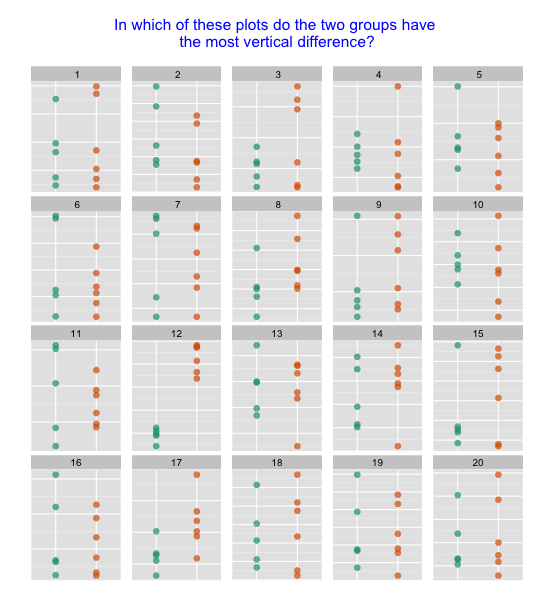
\includegraphics[width=6.5in]{plot_turk9_geno_4_3.png} 
   \caption{A lineup of 20 plots. One of the plots is observed data and rest of the 19 plots are obtained by randomly permuting the group structure. Can you identify the observed data?}
   \label{fig:lineup_geno}
\end{figure}

\subsection{Performance of the observer} Observer who evaluates a lineup do not necessarily be aware of the data underlying a lineup. In response to a specific question the observer is to make a choice based on what he or she sees in the lineup. The choice could be right or wrong depending on whether the data plot is selected or not. Under null hypothesis, all the null plots look similar to what the observed data plot appears to be. This would make it harder to detect the observed data plot in the lineup. It is not expected that an observer would be able to detect the data plot in this scenario. But since there are limited number of plots in a lineup which is 20 in this case, there is a 1/20 chance that the observer would pick the actual plot. This proportion is associated with the type-I error probability. On the other hand if null hypothesis is not true, the observed plot would be different than the null plots making it easier to be distinguished. When multiple observers evaluate a lineup, the proportion of correct response can be used to estimate the power of the visual test \citep{majumder:2013}. 

For a lineup with fixed difficulty, the proportion correct responses may vary for different observers. If an observe evaluates multiple lineups, the proportion of correct evaluations by the observer could be used as a measure of performance by an observer. The another way of measuring the performance of the observer could be the time taken by an observer to evaluate a lineup. Since performance would also depend on the lineup difficulty it is essential to adjust for this before estimating the observer performance.

Some of the factors that may affect the performance of the observer are discussed in Section \ref{sec:factor_performance}. In this paper we focus on estimating the learning effect of the observer in terms of both proportion correct and time taken to evaluate a lineup through the attempts made during the evaluation of multiple plots. We also estimate the location effect of the observed data plot in a lineup.  The other factors are controlled in simulation experiments so that learning effect and location effect can be estimated.

This paper is organized as follows; Section \ref{sec:factor_performance} describes some of the factors that may affect the performance of the observer. Section \ref{sec:exp_design} describes the design of the simulation experiments and methods to estimate the learning trend of the observer and location effect of the observed plot in a lineup. Section \ref{sec:result_socio} presents the analysis of the experimental data and the results.


\section{Factors Affecting the performance of the observer} \label{sec:factor_performance} 

A brief description of the factors that may affect the power of visual inference.

\subsection{Signal in the data}

The power can be estimated from the proportion of correct evaluations. Thus power could be used as a measure of performance of the observer.


\subsection{Choice of Visual Test Statistic} Visual test statistics as defined in \citep{majumder:2013} serve two main purposes. One is to display a prominent pattern that should direct the human observers to select the actual plot in the lineup when the null hypothesis is not true. The another feature is that it should not show any strange pattern when null hypothesis is true, i.e., it should show similar pattern that null plots may have. Thus a visual test statistic is highly associated with the hypothesis. To achieve these purposes it is very important to decide which plot type and plot features should be adopted. As discussed in \citep{majumder:2013} following grammar of graphics developed  by \citet{wilkinson:1999} and later improved by \citet{hadley:2009} can give the task a standard control. 

Some of the effective features of visual test statistics are discussed in \citep{heike:2012} including plot type, color and shape of the plots. It is also observed that a scatterplot may do a better job than a box plot when using as a visual test statistic for regression parameters \citep{majumder:2013} .  \citep{niladri:2012} presents some \textit{distance measure} to determine how a plot may be different from another.

Plots to do: for the same signal strength show the proportion correct for scatterplot and boxplot. eg., qplot(effect, ump-visual power, color= plot-type)

\subsection{Question that Human Observer Answers} When a observer is prepared to evaluate a lineup, there needs to be a guideline what exactly should be looked for in a lineup. The researcher knows about the hypothesis but the observer does not know the underlying details of the lineup. Thus the researcher needs to ask a question observer is to answer while evaluating the lineup. This question should provide the observer a little clue so that the answer reflects the hypothesized patterns in the actual plot. For example Table \ref{tbl:visual_stat} shows the questions asked for the simulation experiments done by  \citet{majumder:2013}. Notice that for case 1 if the observer can identify the actual plot in the lineup that should indicate that the plot chosen has the most vertical difference between groups A and B which is exactly what the researchers intend to examine. Similarly for case 2, a correct evaluation would indicate that the slope is different than the slope that may show up just from randomness.


\begin{table*}[hbtp] 
\caption{Visual test statistics and question asked to the observers to answer while evaluating a lineup } 
\centering 
\begin{tabular}{m{0.5cm}m{2cm}m{3cm}m{7.5cm}} 
\hline\hline 
Case & Statistic & Test Statistic & Lineup question \\ [0.5ex] % inserts table %heading 
\hline 
1  & Box plot & \begin{minipage}[t]{3cm} 	\scalebox{0.45}{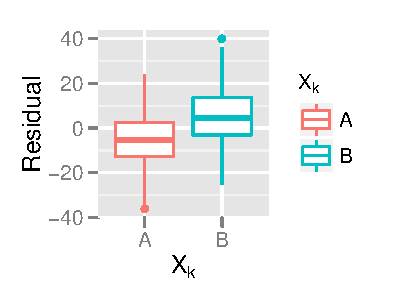
\includegraphics{stat_category.pdf}} \end{minipage} & Which set of box plots shows biggest vertical difference 
between group A and B? \\
2 &  Scatter plot & \begin{minipage}[t]{3cm}   \scalebox{0.45}{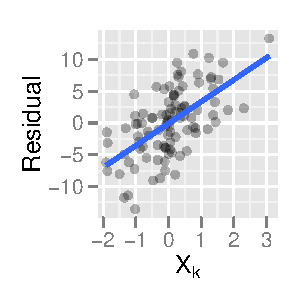
\includegraphics{stat_beta_k.pdf}}\end{minipage} & Of the scatter plots below which one shows data that has steepest slope? \\ 

\hline 
\end{tabular} 
\label{tbl:visual_stat} 
\end{table*} 

These questions are very crucial for the power of visual test. They help observer think in a controlled direction. Notice that there may be unnecessary patterns in the actual data plot which may not necessarily indicate the existence of the significant signal in the plot. These question help observer not to be misguided by those patterns. To review further on this \citet{majumder:2013} have also asked why the observers choose a specific plot. 



%\subsection{Observer Personality} 

\subsection{Visual Perception of Human Eye} Different people observe the lineup in different ways.  With the help of eye-tracking equipment \citet{zhao:2012} track the observers' eyes to see how they go through the plots in a lineup to come to their answers. The result suggest that people have particular methods of reading lineups. Some people read lineups from left to write direction while some read from upward to downward. Some people start looking from the center of the lineup while others start from the top left corner. In the earlier phase of the exercise, the observer tend to scan the plots and then start comparing plots to make a final decision. Beside right-left or up-down directions observer show some diagonal movement too. 

Given this pattern of human eye tracks, it may effect the performance of an observer depending on where the actual plot is placed in the lineup. If the actual plot is on the top left corner and the observer starts from that point it may be easier to detect the actual plot earlier in the exercise and the observer could get plenty of time to make comparison. Thus the position of the actual plot in a lineup has some impact.

\subsection{Demographics of Observer}  Age, gender and location of the observer.

\subsection{Individual Performance of the Observer} Each person is different from others in some way. For example, in a controlled experimental study \citet{zhao:2012}  notice that some people spend a lot of time to decide no matter whether the lineup is difficult or easy while some simply glance at lineups to make a decision. This influences the response of the observer and we see the subject specific variation in the power of visual test \citep{majumder:2013}. 

\section{Simulation Experiment and Methods}\label{sec:exp_design}
The performance of the observer while evaluating a lineup would depend on the factors described in Section \ref{sec:facotr_performance}. In this section we present the experimental design to control some  of them so that learning effect of observer and location effect of a plot in the lineup can be estimated.

\subsection{Experiment Setup} Description of the simulation experiment giving focus on demographics and skills of experimental subjects.

\begin{table}[hbtp]
\caption{Amazon mechanical turk experiments and their properties. Duration in hours per 100 tasks show the popularity of some tasks compared to others.}
\centering
\begin{tabular}{rlrrrrrrr}
  \hline
& Experiment& \multicolumn{2}{c}{ Total Task}& Average & \multicolumn{2}{c}{Duration (hour)} & Payment & Pay rate\\
\cline{3-4} \cline{6-7}
Serial & description & submitted & rejected & time(min) & Actual & 100 task& \$/task & \$/hour\\ 
  \hline
1 & Boxplot & 406 & 106 & 10.68 & 146.48 & 36.08 & 0.50 & 2.81 \\ 
  2 & Scatterplot & 359 &   9 & 10.80 & 42.68 & 11.89 & 1.00 & 5.58 \\ 
  3 & Contaminated plot & 219 &  19 & 13.53 & 126.17 & 57.61 & 1.00 & 2.22 \\ 
  4 & Polar vs Cartesian & 110 &  10 & 20.65 & 11.65 & 10.59 & 1.00 & 2.91 \\ 
  5 & Hist vs density & 234 &  37 & 17.85 & 41.57 & 17.76 & 1.00 & 3.36 \\ 
  6 & Violine vs boxplot & 417 &  17 & 17.95 & 105.87 & 25.39 & 1.00 & 3.34 \\ 
  7 & Group separation & 106 &   6 & 16.13 & 5.15 & 4.86 & 1.00 & 3.72 \\ 
  8 & Sine Illusion & 101 &   1 & 16.52 & 78.38 & 77.60 & 1.00 & 3.63 \\ 
  9 & Gene expression & 103 &   3 & 12.47 & 11.27 & 10.94 & 0.50 & 2.41 \\ 
  10 & Test normality & 406 &   6 & 22.70 & 74.35 & 18.31 & 1.00 & 2.64 \\ 
   \hline
\end{tabular}
\label{tbl:mturk}
\end{table}


\begin{figure}[htbp] 
   \centering
   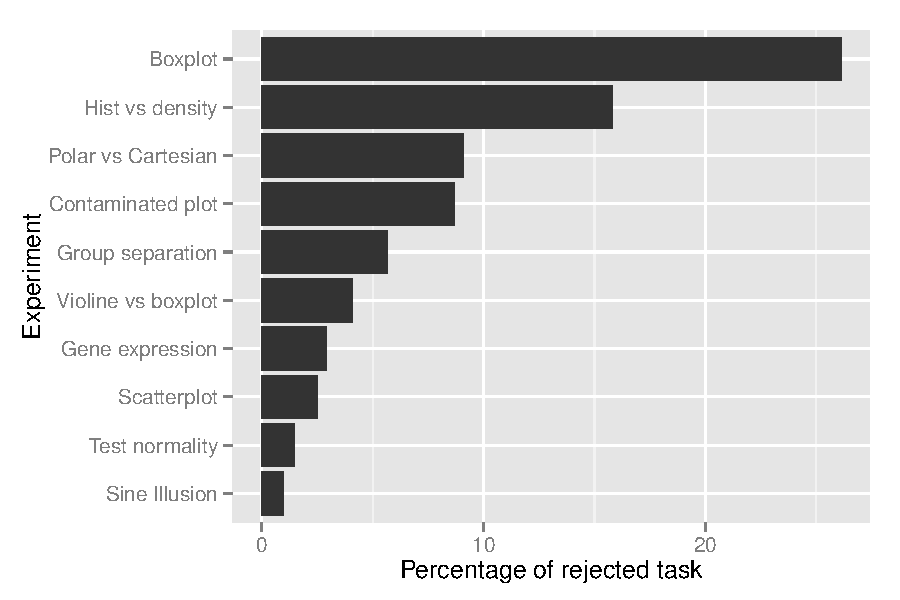
\includegraphics[width=3in]{rejected_task.pdf}
      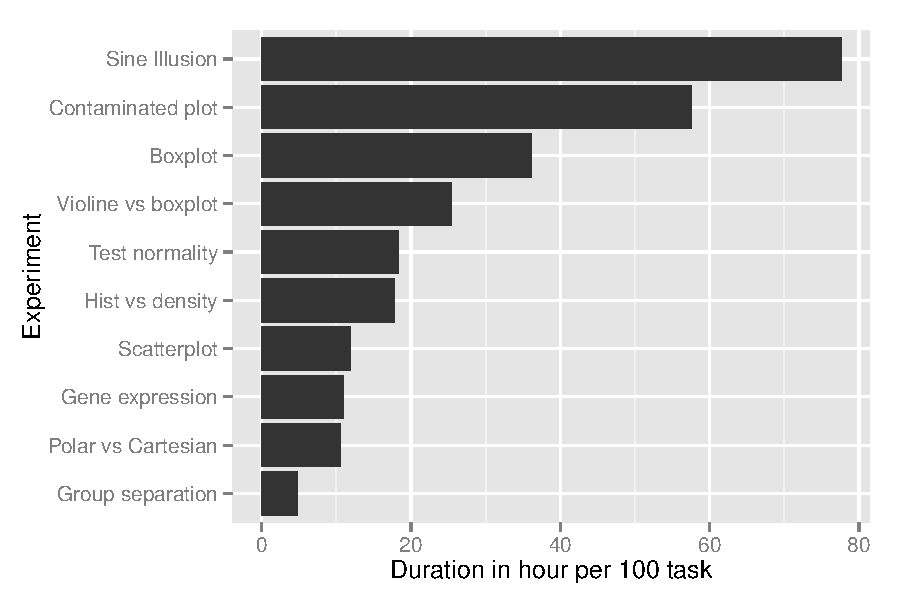
\includegraphics[width=3in]{task_duration.pdf} 
   \caption{Percentage of rejected tasks and duration of each experiment in hour per 100 tasks for each of the 10 experiments. Most of the tasks got rejected for box plot experiment.  Even though the sine illusion experiment took longest to finish the rejection rate is lowest for this experiment.}
   \label{fig:task_duration}
\end{figure}


%\subsection{Estimation of sample size}  How the sample size is estimated
\subsection{Data collection methods}  Description of the simulation experiment giving focus on demographics and skills of experimental subjects.
\subsection{Amazon Mechanical Turk}

Amazon Mechanical Turk \cite{turk} or MTurk is an online work place where people from around the world can perform some tasks and get paid. Usually tasks are very simple and no specialized training is required. Being a human is the main requirement. Tasks are designed for anyone to do but some tasks may require that workers satisfy some skill level depending on the recruiters need. The tasks are designed such that it does not take much time to complete. Humans are still better than computers in performing these types of tasks. The the amount of money paid for each task is very small as well. 

It is very fast, cheap and reliable to recruit people from MTurk. Thats why it is getting very popular among the researchers who perform human subject experiment. The another benefit is that a very diverse pool of subjects can be recruited which is otherwise very hard to obtain for a study. The researchers can easily filter the workers based on their experimental design, such as recruiting people only from a specific geographical location or a group of people who satisfy certain criteria etc. The recruiter can decide who they pay or not. Workers have to satisfy the task requirement to ensure payment. But at the end it is the recruiter who has the final say. Usually recruiters pay promptly after the task has been done properly and thats why MTurk is very popular among the online job seeker. At any point of time thousands of tasks are available for the thousands of workers around the world. 

Because of its convenience it is getting popular for scientific research study. In comparison with a lab study \cite{suri:2010} perform the same study using MTurk and demonstrate that their study results are as good as the lab study results even though MTurk study required less time and cost while provided more convenience. \cite{majumder:2013} recruited people from MTurk for their simulation study in estimating the power of visual statistical inference. They have done numerous pilot studies in lab before doing actual MTurk study and found similar results. \cite{mason:2012} explains various features of MTurk and describes how it can be used as part of human behavioral study.

\subsection{Model to Estimate Learning Trend}

\subsection{Model to Estimate Location Effect}

\section{Results}\label{sec:result_socio}
\subsection{Overview of the Data}
\subsection{Diversity of the Experimental Subjects} Amazon Mechanical Turk \cite{turk} web site is a good source for recruiting people to evaluation lineups. It is a source of diverse workers who can give us feedback on visual inspection.  Figure \ref{fig:turker_location} shows the location from where we received data. Notice that we received data from around the world and we observed diversity of location in the collected data. We notice diversity in not only location of the observers but also their gender, age groups and education levels. Table \ref{tbl:demographics} shows that number of male and female participants are almost same.

\begin{figure}[htbp] 
   \centering
   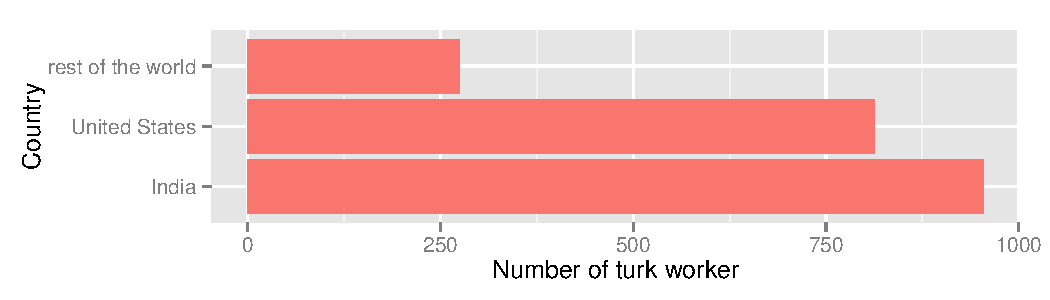
\includegraphics[width=4.5in]{turker_country.pdf} 
   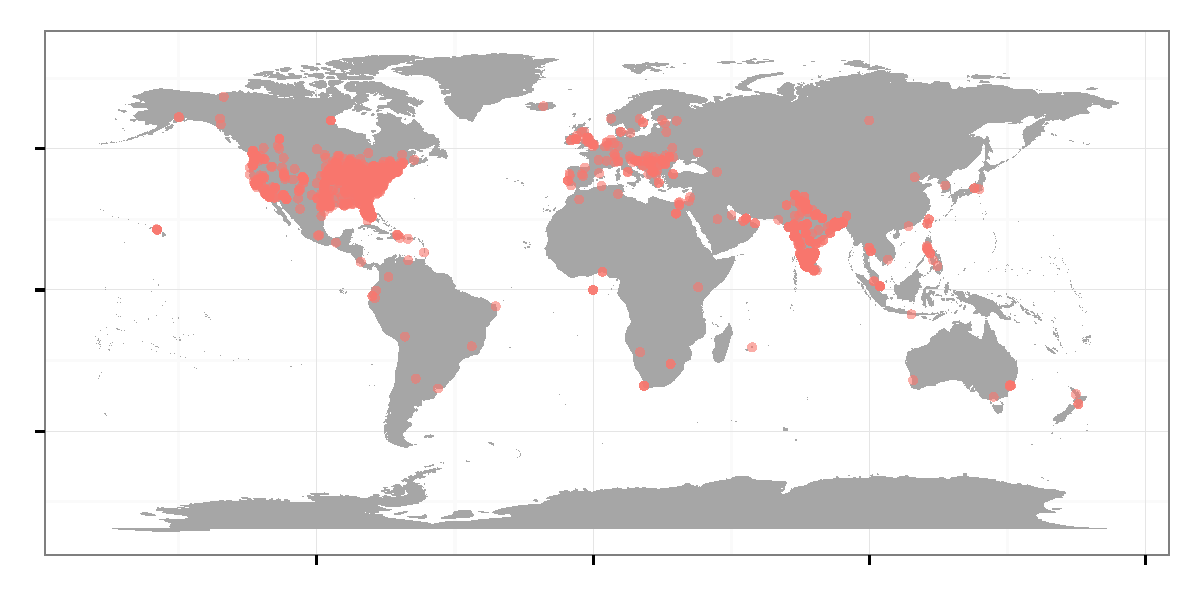
\includegraphics[width=4.5in]{turker_location.pdf}    
   \caption{Location of the Amazon Mechanical Turk workers participating our study. Most of the people are coming from India and United States even though there are people from around the world.}
   \label{fig:turker_location}
\end{figure}

The large number of participants are from age group 18 to 35. Interestingly we see many participants from older age groups as well. Specially for united states almost all the age groups show uniform participations after age 30 as in Figure \ref{fig:demographic_info}. Notice that fewer people participated from India beyond age 40 compared to united states. Even thoug total participations from india is larger compared to United States, they are mostly young people who are capable of using internet and computer. 


\begin{figure}[htbp] 
   \centering
   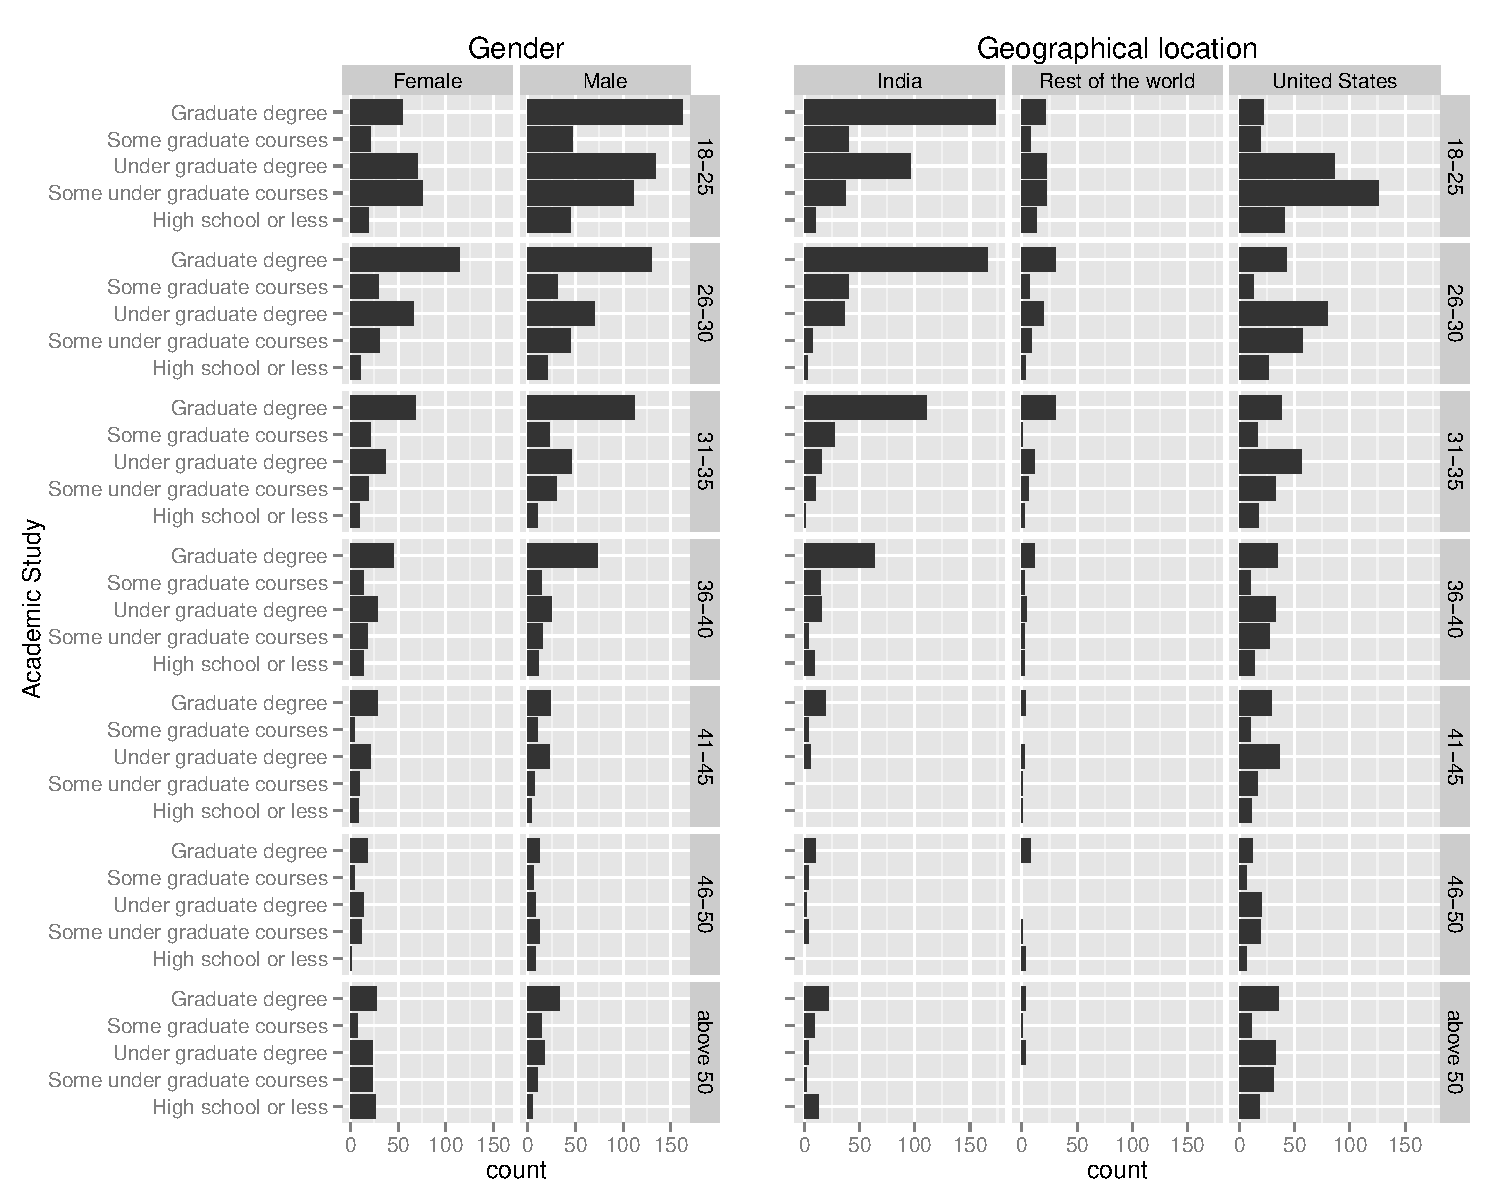
\includegraphics[width=6in]{demographic_info.pdf} 
   \caption{Countrywise distribution of age and academic levels of the MTurk workers participating the experiments shows the diversity of the subjects in all the demographic aspect. Almost equal number of male and female subjects participated the online experiments.}
   \label{fig:demographic_info}
\end{figure}


\subsection{How people pick the data plot} In the experiment setup we have a question for the turk observers to choose the reason for their selection of a particular data plot. It is shown by \cite{majumder:2013} that these choice reasons reveal the way people picks the data plot in the lineup. To investigate this further we added free text input option for their choice reason instead of some fixed reasons to select from. In this experiment people could write whatever they think their reasons for choice are. Figure \ref{fig:wordle} shows the words used to explain their reasons for choice. The most common words used to explain their choice are points and green which indicates two important feature of a plot. One is the indicator of plot aesthetics and the other is the color. Spread, steepest, line and apart are some other important words used frequently. Spread and apart are indicative of variability in the data. Steepest and line indicates some sort of systematic pattern in the data.

\begin{figure}[htbp] 
   \centering
   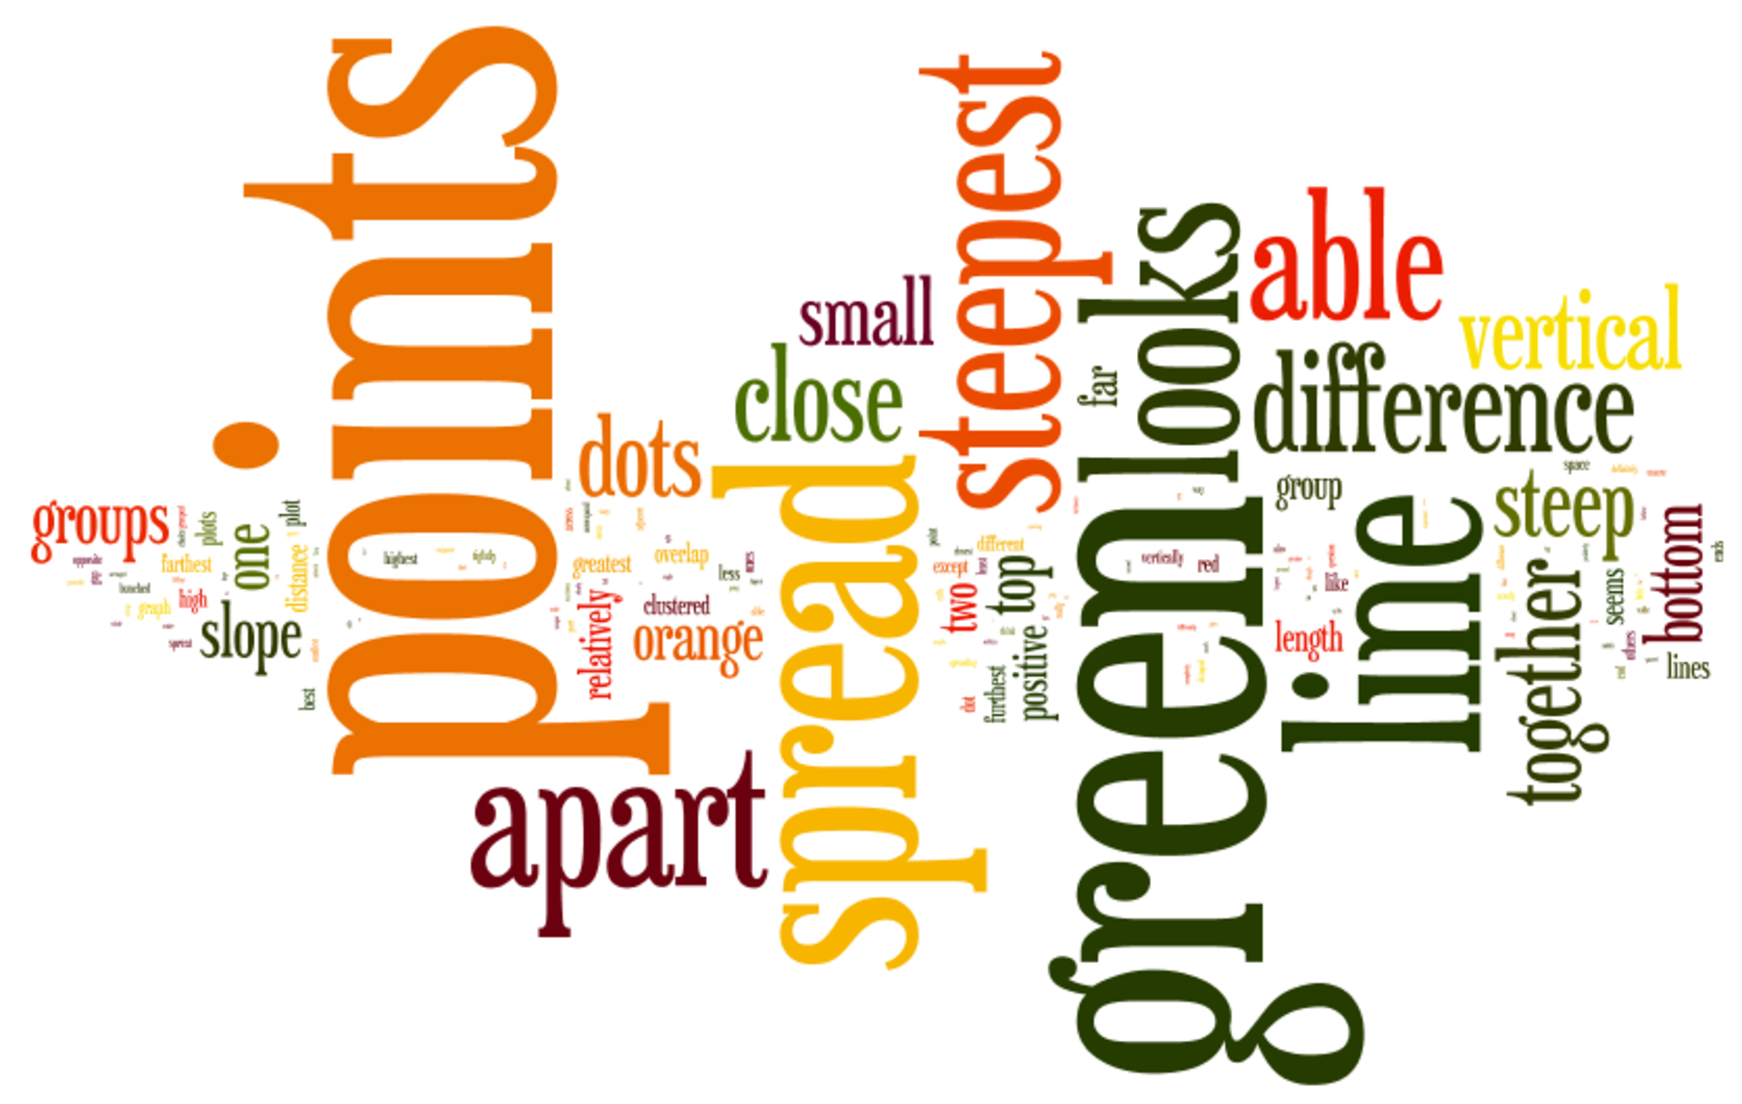
\includegraphics[width=3.5in]{reasoning_words.pdf} 
   \caption{Words used to explain the reasons for selection of data plot in a lineup show what features of a lineup may help a non-statistician to evaluate it. Larger font indicate more people choosing that word. Different color is used just to separate the words.}
   \label{fig:wordle}
\end{figure}

Figure \ref {fig:wordle} also shows some insight about peoples way of reading a plot. We notice that variability in the data, color and aesthetics used to generate plots and existence of any systematic pattern in the plot are some of the important features revealed from the figure. These features are commonly used by human brain to examine and compare plots. Notice that these features may be specific to this particular experiment. There could be different other features people would use to evaluate a lineup depending on the situation. But these words we have a general idea how people may think to evaluate a lineup.

Turk workers are not necessarily trained on statistics or aware of specific terms used in statistics or statistical plots. Thus it is also interesting to note that how they explain things that have specific definitions and meaning. Notice in Figure \ref {fig:wordle} that some keywords like spread, apart should be analogous to larger variability while together,  close may be for indicating smaller variability.


\begin{figure}[htbp] 
   \centering
   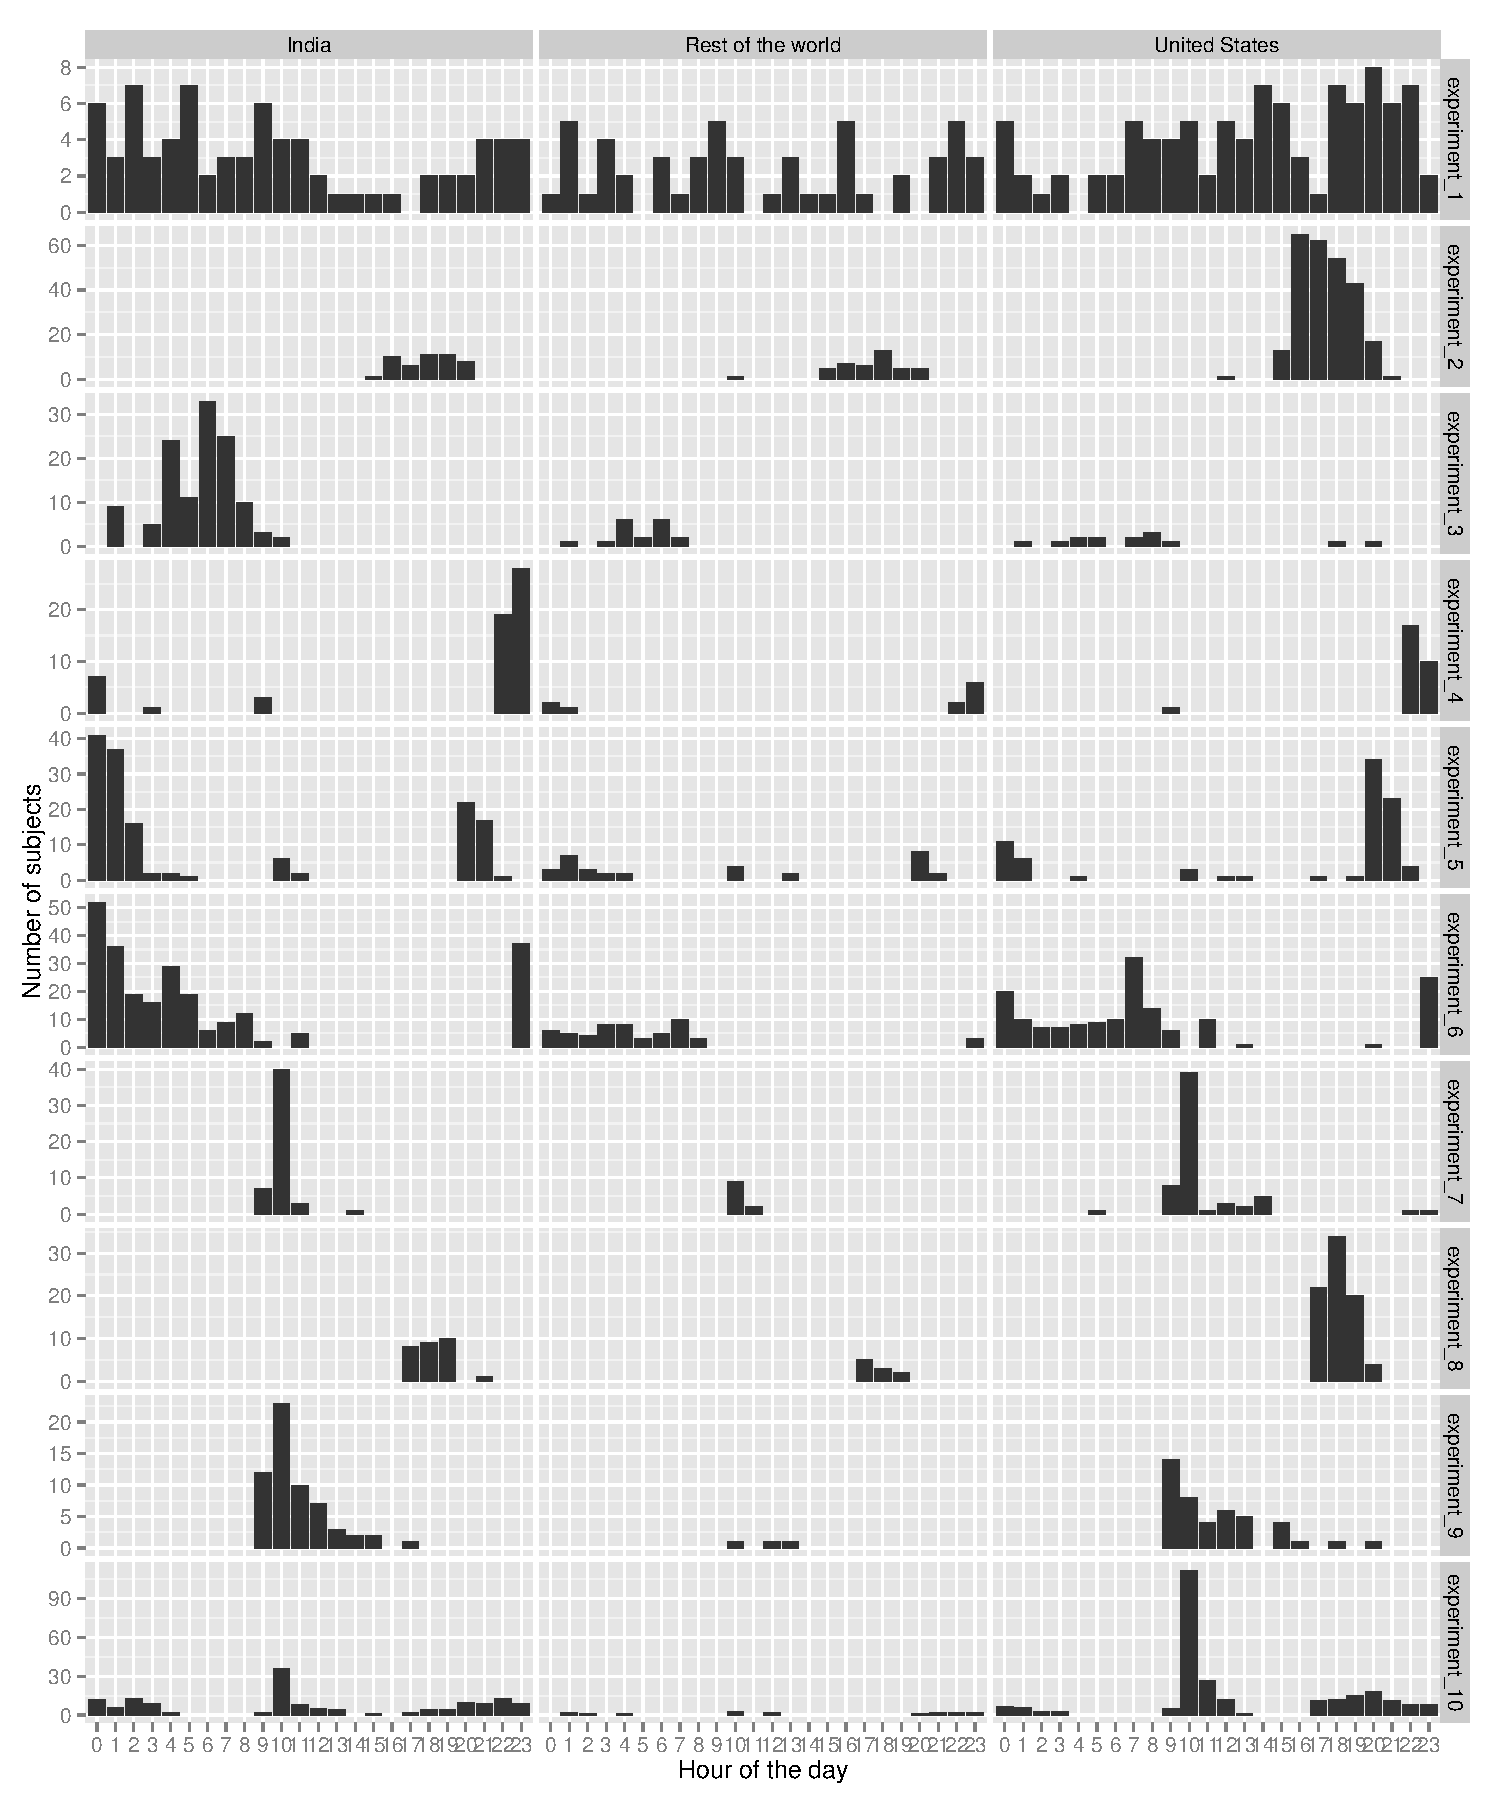
\includegraphics[width=4.5in]{participation_time.pdf} 
   \caption{Time of the day when the participants work. Experiment 1 shows MTurk workers participated the experiments around the clock. Other experiments did not take a whole day to finish.}
   \label{fig:participation_time}
\end{figure}


\subsection{Learning Trend of the Observer} Each subject participating the experiment has seen multiple number of lineups for evaluations. Suppose $K$ be the number of lineups evaluated by a subject and $A_k$ be the $kth$ attempt, $k=1,2, ..., K$. Subjects may have a chance for self learning and do better on lineups shown later in the sequence. They may learn from their previous mistake or they may learn about the features of the plots being evaluated as they progress. Thus if there is any learning trend that should be apparent in proportion correct over $A_k$. But to obtain this we have to adjust for lineup difficulty and individual performances.

To accomplish this we fit generalized mixed effect model presented in \cite{majumder:2013} with lineups and subjects as random effect and no fixed effect. This gives the estimation of proportion correct responses  and we obtain residuals of the fitted model. The residuals give variations in proportion correct adjusted for lineup difficulties and individual skills. If there is any learning trend over different attempt $A_k$, the residuals should have that information since $A_k$ was not included as a covariate in the model. %At this point we focus on absolute residuals over different attempts to study the deviations due to attempts. An smaller absolute residual at attempt $A_k$ should indicate learning from all other attempts less than $k$. 

A plot of residuals against the attempts $A_k$ should reveal the trend if there is any. Figure \ref{fig:learning_trend} shows such plots for three experiments naming experiment 5, 6 and 7. For all the experiments we see some increasing trend of the residuals. This could be attributed to the exhaustion of subjects' attempt after some earlier evaluations are made.  But none of apparent trend are statistically significant. 

%covariates attempt number and $p$-value of the lineup. The $p$-value of the lineup measures some sort of difficulty and including this should adjust for the difficulty level of the lineup while estimating the probability of correct responses in each attempt. Figure \ref{fig:learning_trend} shows the fitted subject wise learning pattern as well as overall learning pattern for each of the experiments. The parameter estimates of the model are shown in Table \ref{tbl:model_par}.


\begin{figure}[htbp] 
   \centering
   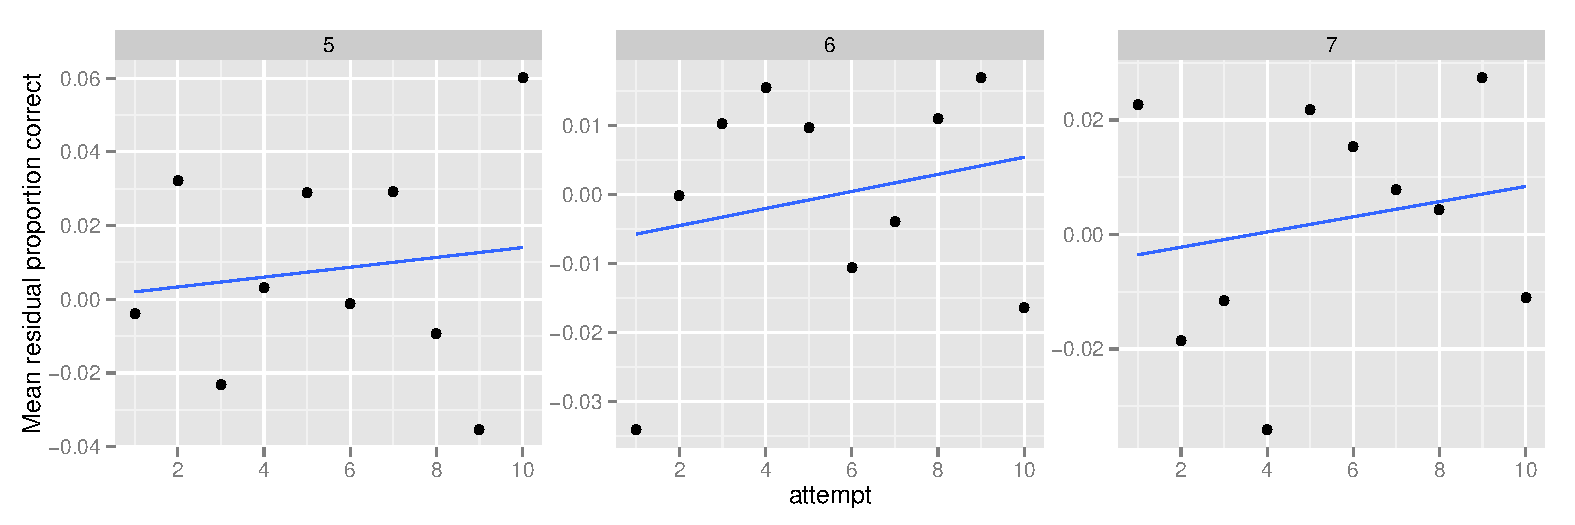
\includegraphics[width=6.5in]{learning_trend.pdf} 
   \caption{ Mean residuals of proportion correct vs attempt obtained by adjusting for lineup and subject specific variation. For experiment 5, we see a downward trend which may indicate some learning as attempt progress, but none of the slopes in these three experiments are statistically significant.}
   \label{fig:learning_trend}
\end{figure}

Learning trend is not only related to the proportion correct responses. It may be possible that people learn to answer fast. We examine this by the time taken for each evaluation. We fit a mixed effect linear model with time taken considering lineup and subjects as random effect. The resulting residuals are plotted in Figure \ref{fig:learning_trend_time}. It appears that in the later attempts observers take less time to evaluate a lineup. Even though it does not tell much about improving their performance over attempts, but it does indicate the improvement of their evaluation skill. Adding this information with what we observe in Figure \ref{fig:learning_trend}, we can say that the observers' improved skills could not contribute to their performance. It only help them finish the task faster in later attempts.

\begin{figure}[htbp] 
   \centering
   
\includegraphics[width=6.5in]{learning_trend_time.pdf} 
   \caption{Mean residuals of time taken vs attempt obtained by adjusting for lineup and subject specific variation. For all the experiment the downward slopes indicate that MTurk workers take less time as they progress through their attempts.}
   \label{fig:learning_trend_time}
\end{figure}


\subsection{Location Effect of Data Plot in the Lineup}

We set up a Turk experiment to examine whether there is any difference of performance based on the location of actual data plot in the lineup. For this five locations of a lineup were randomly chosen to put the same actual data plot. The locations are 2,9,12,16,20 for Interaction effect and 1,8,12,17,20 for Genotype effect. For a lineup with specific data plot location, five sets of null plots are used giving 5 lineups for each location. In total we have 25 lineups for Interaction effect and 25 lineups for Genotype effect. These 50 lineups are then evaluated by 100 people recruited from Amazon Mechanical Turk. Each person evaluated 3 lineups one from Interaction, one from Genotype and the third one was a test lineup. The test lineup is used to process the payment and examine the quality of the data and the responses of the test plot is not added to our analysis. 

The proportion of correct responses by the turk observers are shown in Figure \ref{fig:location_effect}. Notice that the data plot is same for each location but we see some variability of performance based on different null plots. This may happen if some null plots appear to be more similar to the actual plot while the others are not making some lineups harder than others even though the actual data plot is same. This pattern is evident in the Figure \ref{fig:location_effect} as we see proportion correct for null plot 5 is consistently above the null plot 1 for each of the locations. But this variability could be controlled at some extent by collecting more data for each location. Since the variability is larger when we have small number of responses as we see in the figure. For example, we have only one response for null plot 3 and 5 for Interaction effect which should lead to the extreme proportion of correct since one response would either be correct or wrong. 

\begin{figure}[htbp] 
   \centering
    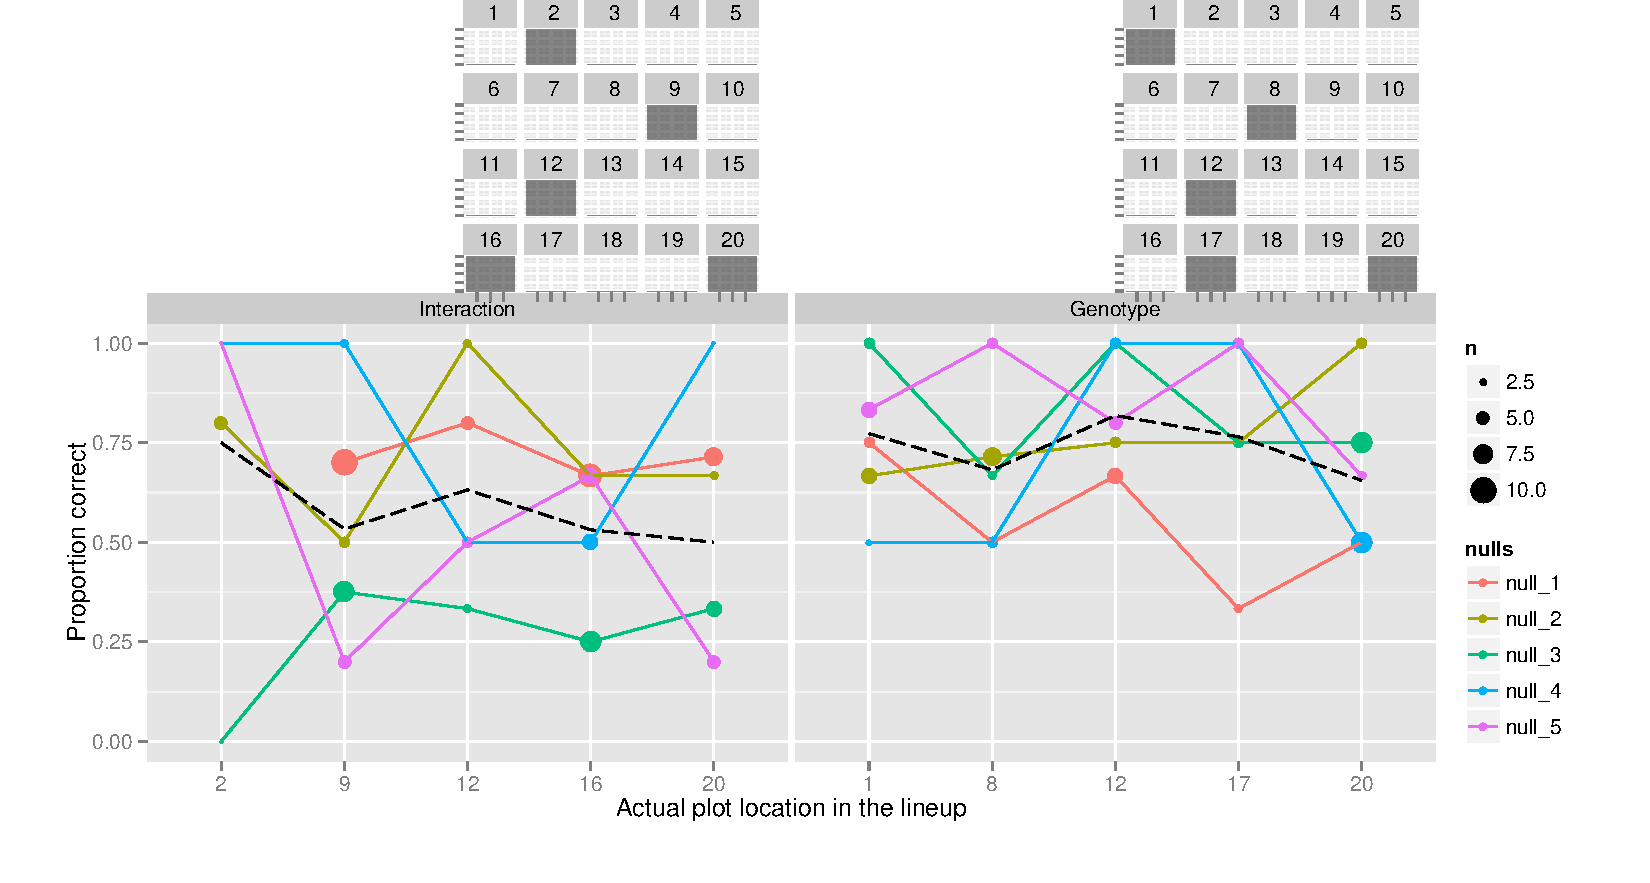
\includegraphics[width=6.5in]{proportion_nulls_guide.pdf} 
   \caption{Location of data plot in the lineup and proportion correct for both Interaction and Genotype effect. Each colored line represents a null set and the size of the dots represents number of responses. The overall average proportions are shown by dashed line. The actual data plot locations are shaded grey on the top panels to demonstrate their relative positions on a lineup.}
   \label{fig:location_effect}
\end{figure}

It is also interesting to check whether the proportion correct differs if the actual plot is on the outer boundary of the lineup or inside the outer boundary. As we see in Figure \ref{fig:location_effect}, location 9, 12 are inside for Interaction effect and location 8, 12 are inside for Genotype. It does not appear to have any difference whether the actual plot is inside or outer border of the lineup.

The overall proportion of correct response does not seem to vary much for different location indicating the non-existence of location effect. Since the actual data plot is same for each of the null sets of plot, the response data constitutes a multivariate response. Thus, to examine if the difference in proportion correct among the locations is statistically significant we fit a one way multi variate analysis of variance (MANOVA) model to the data.

 Suppose $Y=(Y_1,Y_2, ... , Y_p)$ is a vector of random variable with dimension $p=5$ representing the response for five null sets. let $Y_{ij}$ represents $jth$ vector response for $ith$ location with $i=1,2, ..., 5$. We fit the following MANOVA model 
\begin{equation}\label{manova}
Y_{ij} = \mu_{i} + \epsilon_{ij}
\end{equation}
where $\mu_{i}= (\mu_{1i},\mu_{2i}, ..., \mu_{pi})$ is the mean vector for location $i$ and $Var(\epsilon_{ij})=\Sigma$. 

Model \eqref{manova} enables to test if the mean vectors are similar for different locations. To fit the model we use anova function of stats package of \cite{R:2012}. The results are shown in Table \ref{tbl:manova}. The $p$-values for both Interaction and Genotype effect are much bigger than the conventional threshold of 0.05 and we failed to reject the hypothesis that there is no difference in location. 

\begin{table}[hbtp]
\caption{The results obtained by fitting MANOVA Model \eqref{manova}.}
\begin{center}
\begin{tabular}{ccccccccc}
  \hline \hline
 Location & && & \multicolumn{3}{c} {Degrees of Freedom}  & F test \\
 \cline{5-7}
 Effect & DF & Pillai & Approx. F & Numerator& Denumerator &Residual & p value\\
  \hline
  Interaction& 3&1.4783 &0.7772&15&12 & 6 & 0.6821 \\ 
  Genotype &4&1.7796 &1.1221&20&28 & 8 &  0.3824 \\ 
   \hline
\end{tabular}
\end{center}
\label{tbl:manova}
\end{table}

We also fit Model \eqref{manova} with only two locations based on outer or inner plot location. By outer location we mean the data plot location which is on the border area of the lineup. For example inner locations of a lineup would be 7,8,9,12,13,14. It turns out that inner and outer locations are also not significantly different.





%% latex table generated in R 2.15.0 by xtable 1.7-0 package
%% Fri Sep  7 10:28:47 2012
%\begin{table}[hbtp]
%\caption{Fixed effect parameter estimates of generalized mixed model. Note that attempt is not significant for experiment 2. The continuous covariate, lineup difficulty, was measured by the $p$-value of the actual plot in the lineup.}
%\begin{center}
%\begin{tabular}{llrrrrl}
%  \hline
%& Parameters & Estimate & Std..Error & z.value & P-value  & \\ 
%  \hline
%\multicolumn{2}{l}{\bf{Experiment 1} } &&&& &\\
%&(Intercept) & -0.30 & 0.10 & -2.89 & 0.00 & ***\\ 
% & attempt & 0.08 & 0.02 & 4.21 & 0.00 & ***\\ 
% & lineup difficulty & -11.32 & 1.01 & -11.19 & 0.00 & ***\\ 
%\multicolumn{2}{l}{\bf{Experiment 2} } &&&&& \\
% & (Intercept) & 2.36 & 0.15 & 16.09 & 0.00 & ***\\ 
% & attempt & 0.01 & 0.03 & 0.35 & 0.72 \\ 
% & lineup difficulty & -55.03 & 2.20 & -25.00 & 0.00 & ***\\ 
%\multicolumn{2}{l}{\bf{Experiment 3} } &&&& \\
% & (Intercept) & 0.25 & 0.16 & 1.58 & 0.11 & .\\ 
% & attempt & 0.10 & 0.03 & 3.34 & 0.00 & ***\\ 
% & lineup difficulty & 3.00 & 0.56 & 5.36 & 0.00 & ***\\ 
%   \hline
%\end{tabular}
%\end{center}
%\label{tbl:model_par}
%\end{table}

% \footnote{Signif. codes: 0 �***� 0.001 �**� 0.01 �*� 0.05 �.� 0.1}



\section{Conclusion}

\appendix

\begin{table}[hbtp]
\caption{Demographic information of the subjects participated the MTurk experiments.}
\centering
\begin{tabular}{rlrrr}
  \hline
 & levels & subsjects & avg\_time & response \\ 
  \hline
Gender & Male & 1348 & 48.51 & 13493 \\ 
   & Female & 991 & 43.75 & 10564 \\ 
\hline
  Education & High school or less & 193 & 37.21 & 2241 \\ 
   & Some under graduate courses & 418 & 42.84 & 4070 \\ 
   & Under graduate degree & 584 & 44.29 & 5775 \\ 
   & Some graduate courses & 245 & 43.43 & 2460 \\ 
   & Graduate degree & 902 & 52.18 & 9511 \\ 
\hline
  Age & 18-25 & 740 & 42.97 & 7311 \\ 
   & 26-30 & 547 & 46.27 & 5585 \\ 
   & 31-35 & 376 & 44.27 & 3923 \\ 
   & 36-40 & 257 & 55.03 & 2714 \\ 
   & 41-45 & 141 & 43.90 & 1519 \\ 
   & 46-50 &  95 & 49.29 & 1003 \\ 
   & 51-55 &  83 & 48.67 & 867 \\ 
   & 56-60 &  64 & 59.73 & 678 \\ 
   & above 60 &  38 & 48.67 & 457 \\ 
   \hline
\end{tabular}\label{tbl:demographics}
\end{table}


\bibliographystyle{asa}
\bibliography{references}

\end{document}



